% $Id: gui_bmodel.tex 395 2011-11-17 22:34:59Z cphillip $

\chapter{Computing Feature and Region Contributions}
\label{chap:ComputeWeights}

\minitoc

\section{Introduction}

The previous module allows the user to specify one or more models. These include the machine to be used, the cross-validation scheme and the classification/regression problem. The estimation of those models led to predictions on unseen/test data (in each fold), from which measures of performance of the model can be derived.

In addition, as PRoNTo uses linear models it provides the option of recovering the model weights in the original feature (voxel) space, and transforming the weights vector into an image, or map. These maps contain at each voxel the corresponding weight of the linear model (together defining the optimal decision function), and which related to how much this particular voxel contributed to the classification/regression task in question. The weights can later be displayed using the `Display results' module (described below).

Furthermore, the MKL machine estimates contribution of each kernel to the final decision function. This means that there will
be one value per region of interest as defined by an atlas and/or per modality (depending on how multiple kernels were built).
Therefore, it is possible to build maps at the region level, in addition to the maps at the voxel level. Regions/modalities
can then be ranked according to their contribution. Since L1-MKL is a sparse algorithm (i.e. only some kernels will have a non-null contribution to the model), this eases model interpretation.

\section{Methods}

The output of the linear kernel models in PRoNTo include the coefficients of the dual representation, i.e. the coefficients of the training examples. These coefficients are then multiplied by the training examples to obtain the model weights. The vector of model weights has the same dimensions of the original voxel space, and can therefore be converted to a 3D image. This computation is done for each fold. The resulting 3D images for all folds are then assembled into a single 4D NIFTI file with dimensions [3D x (number of folds + 1)], where $1$ corresponds to an extra 3D image with the averaged weights over all folds. The NIFTI file is saved in the same directory as PRT.mat. In the case of multi-class classification, one image will be built for each class, the index of the class being saved in the image name (e.g. \textit{image\_ name\_ c1.img}). In the case of multiple modalities being considered as multiple kernels (i.e. not concatenated in samples), one image will be built for each modality, the modality name being appended to the image name.

In addition, it is possible to build an image containing the contributions of each region of interest as defined by an atlas (same dimensions as for the voxel weight images). Two options are available:

\begin{itemize}
\item Contributions of kernels estimated through MKL: In this case, the contributions of each region to the model are derived from the contributions of each kernel. This option is available for MKL modelling of feature sets containing multiple kernels based on ROIs defined by an atlas.
\item Summarizing the weights according to ROIs: If a whole brain feature set was used, or if the kernels were added to perform single kernel modelling (e.g. SVM, GP, KRR, RVR), it is possible to select an atlas and summarize a posteriori the weights in each anatomically defined ROI. The contribution of each region is then simply the sum of the absolute values of the weights within that region, divided by the number of voxels in that region (see \cite{Schrouff2013a} for details).
\end{itemize}

In both cases, the contribution of each region is divided by the total contribution of all regions. The derived values can then be seen as percentages of contribution of each region to the decision function. The contributions can be ranked, leading to a list of regions sorted by descending contribution to the model. This list can also be computed if multiple modalities were built and used in an MKL model. In this case, each modality has a contribution to the model, that can be normalized and a sorted list can be derived.

Furthermore, for MKL models - which are sparse in the number of kernels contributing to the model - a bar graph can be built, representing the number of kernels with a non-null contribution to the model. The same graph bar will depict the contribution of each region to the decision function in the case of summarized weights. In this case, the bar graph will not be sparse.

\section{Graphical user interface}

If the user wants to create images of the weights, using the GUI, the user first needs to click the `Compute weights' button
on the main PRoNTo window. This will launch the window shown in Fig \ref{CompWeights}. To estimate the weights and create the
weight maps the user needs to select a {\tt PRT.mat} file. The window is then divided in two panels: a `Feature weights' panel
and a `Atlas-based weights' panel. In the first panel, PRoNTo will show the list of available models, and the user can choose
one model for which to estimate the weights. If the selected model is the MKL modelling of ROI-based kernels, the `Atlas-based
weights' panel will be automatically updated, and the name of the selected atlas at the feature set step will appear.
Otherwise, those fields will stay blank. In the `Feature weights' panel, it is also possible to define the name of the created
image file, which is saved in the same directory as PRT.mat. Alternatively, if left empty, PRoNTo will name the file according to the model name, class (if multi-class machine) and/or modality (if MKL on modalities). The `Atlas-based weights' allows to estimate the contribution of each anatomically defined region to the model. If the model refers to an MKL machine estimated on kernels per region, the `Atlas name' field will be filled automatically and the contribution of each region is derived from the contribution of each kernel. If this is not the case (single kernel machine or feature set), an atlas should be loaded (using the browse option). The weights will then be summarized for each region a posteriori.

\begin{figure}[h!]
\begin{center}
	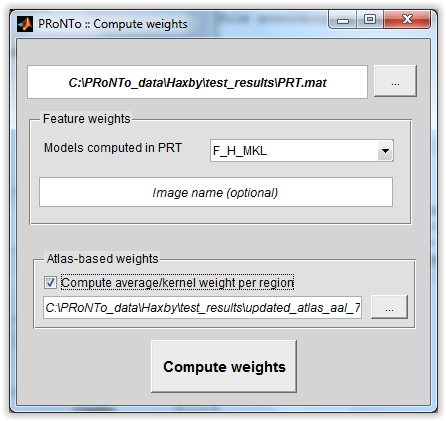
\includegraphics[height=7cm]{images/CompWeights.png}
	\caption{Weights computation GUI.}
	\label{CompWeights}
\end{center}
\end{figure}

\section{{\tt matlabbatch} interface}

The {\tt matlabbatch} module to compute the weights has the same options as the GUI. One main difference being that instead of listing the available models in a given PRT, it will ask for the name (string) of the model to be used. As for estimating models, the name of the model should be exactly the name given in `Specify model'. Another difference is that the batch allows to compute weight images for each permutation. In this case, only the average across folds will be saved in a nifti. This potentially allows for statistical tests to be performed on weights and/or on the derived ranking of the regions (for MKL modelling of anatomically defined ROIs).

\begin{figure}[h!]
\begin{center}
	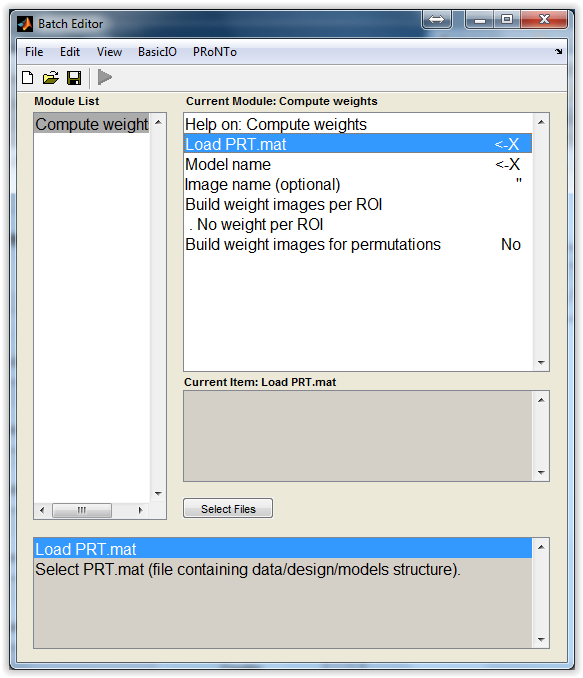
\includegraphics[height=7cm]{images/batchWeights.PNG}
	\caption{Weights computation GUI.}
	\label{batch_CompWeights}
\end{center}
\end{figure}
